\section{Use Cases}
\label{sec-usecases}
%\section{Other Forms of Reuse}
%\label{sec-other}
The combination of low price and abundant capabilities makes discarded phones
suitable for many other forms of reuse. 
We describe two sensing applications using discarded smartphones that we are
currently investigating.
\subsection{Outdoor Monitoring}
\label{sec-rooftop}
\begin{figure}[t]
  \centering
  \subfigure[Outdoor Monitoring]{
    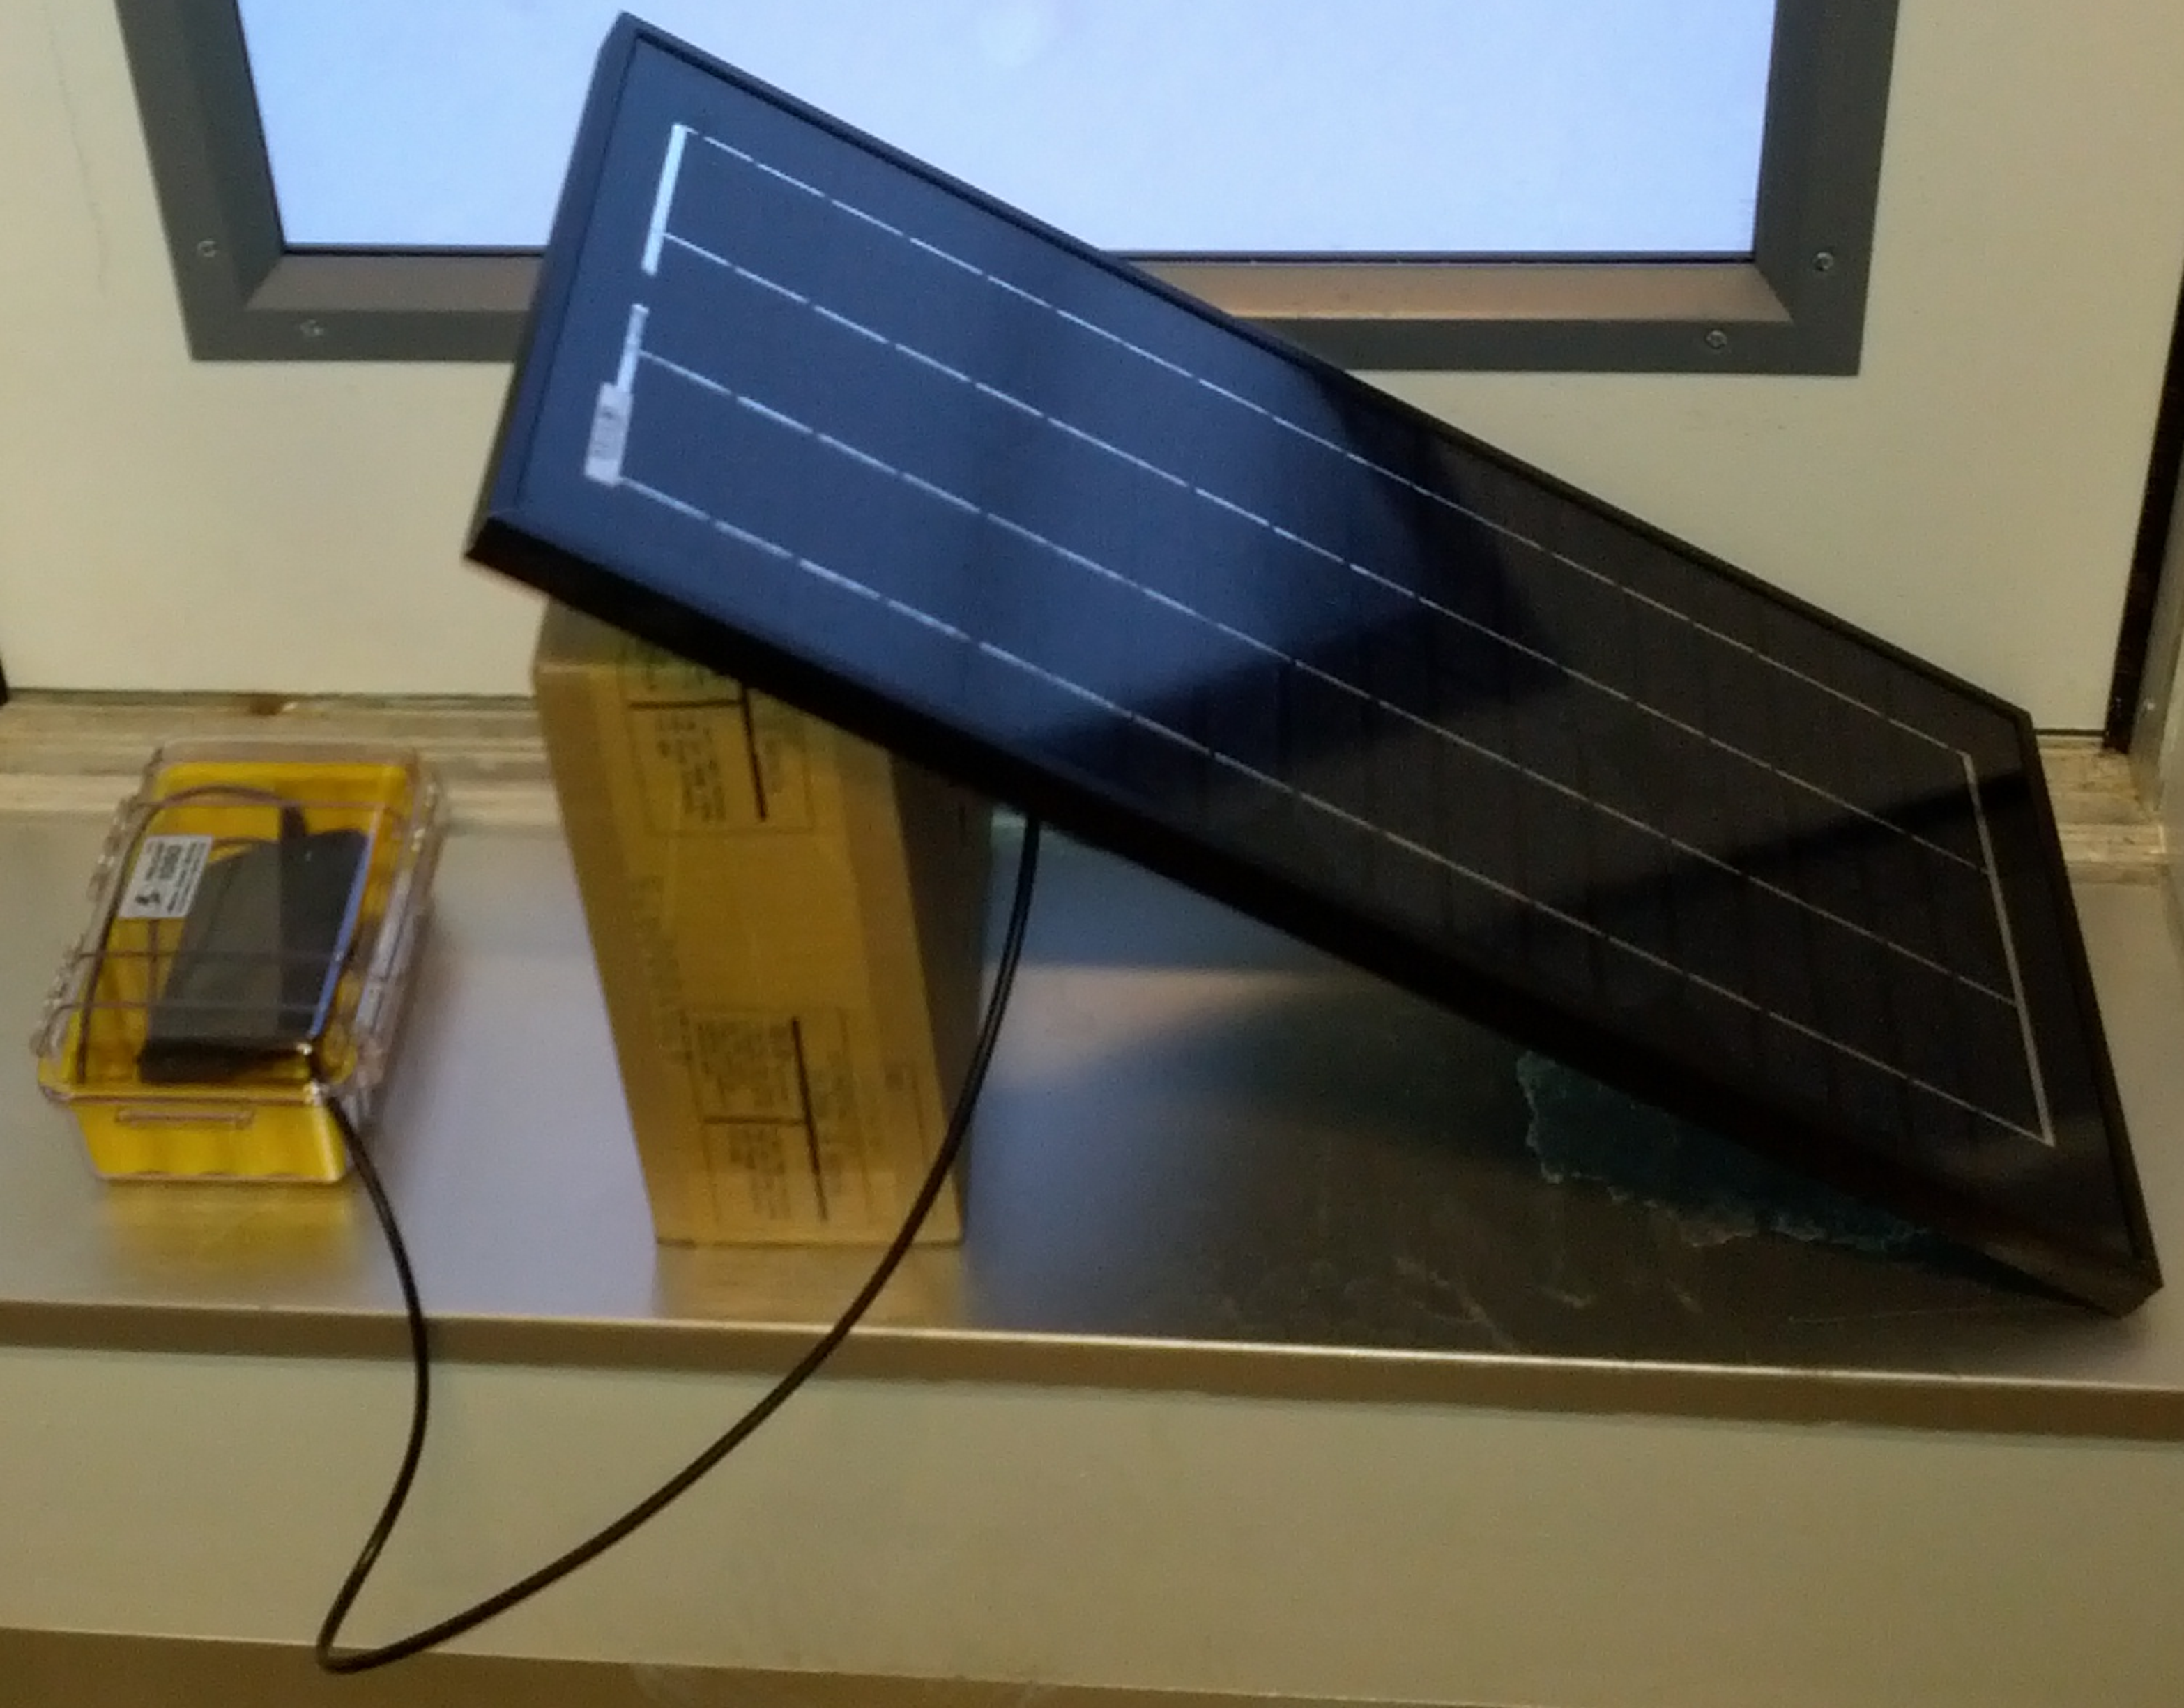
\includegraphics[width=0.45\columnwidth]{./figures/mocksetup.pdf}
  \label{fig-solarsetup}}\quad
  \subfigure[Urban Monitoring]{
    \includegraphics[width=0.45\columnwidth]{./figures/urban1.pdf}
  \label{fig-urbanmonitor}}

  %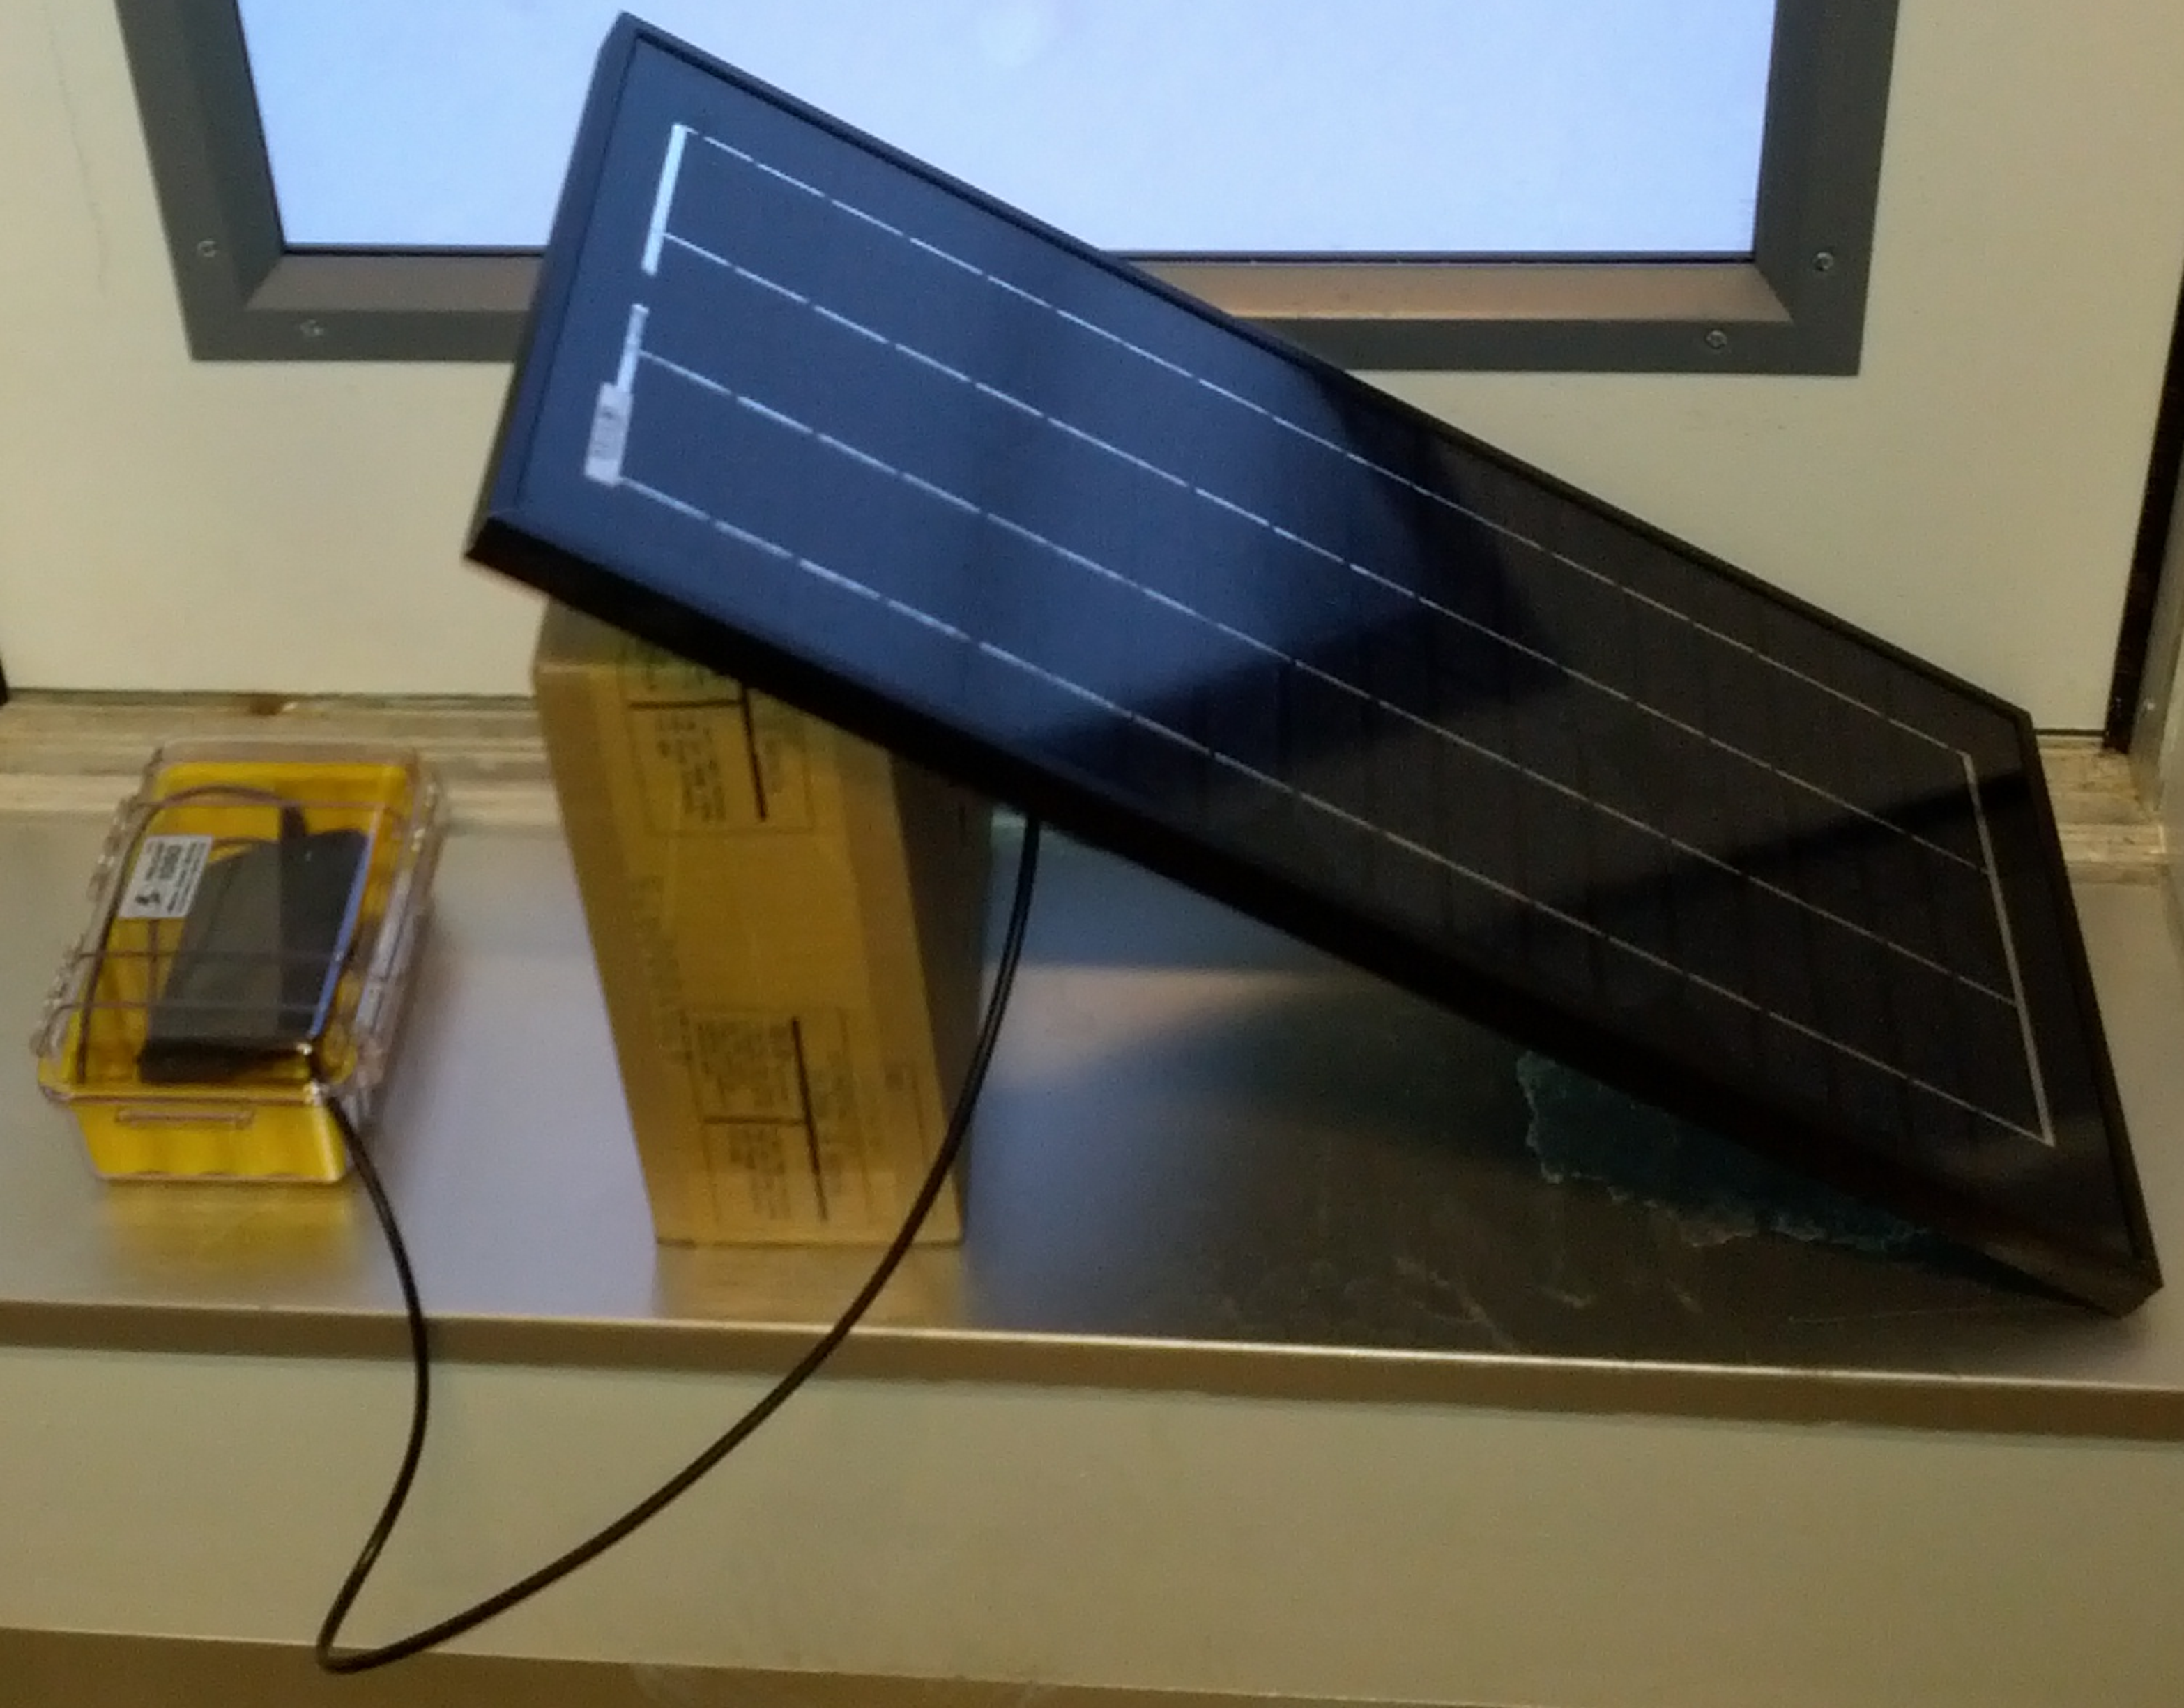
\includegraphics[scale=0.1]{./figures/mocksetup.pdf}

  \vspace*{-0.1in}

  \caption{\small Sensing applications.
  \textnormal{Two of the sensing applications we are currently investigating.}}

  \vspace*{-0.1in}

  %\label{fig-solarsetup}
\end{figure}
Building rooftops can be equipped with discarded smartphones to monitor the
environmental conditions. This in turn can be used to regulate the lighting and
temperature inside the buildings to minimize the energy costs.
Due to the unavailability of power sources on rooftops and the hazardous nature of
power extension cables, it is unviable to deploy smartphones as monitoring
instruments without any power supplies to charge the battery.
Based on our experiments, we think this can be made possible by using other
alternate renewable energy sources like solar energy.

Figure~\ref{fig-solarsetup} shows our current deployment. The solar panel trickle
charges the smartphone battery. The application running in the smartphone
periodically senses the temperature and light levels. It then transmits the
sensed values to a central server every \textit{transmit} interval, a
configurable parameter, using 3G. 

Our initial measurements indicate that a 1800mAH battery can be fully charged
in 25
hours in heavily shadowed areas using the solar panel shown in Figure
~\ref{fig-solarsetup}, such a setup is
enough for a self sustaining monitoring application. The total cost for the
deployment was \$67 excluding the cost for the smartphone and data services.

\subsection{Urban Monitoring}
Cars manufactured post 1996 are equipped to provide On-Board Diagnostics(OBD)
data following the OBD-II specification. With ODB-II, we can extract rich
sensor data from the sensors deployed in the cars. With this data, we can design number of
applications like urban traffic monitoring, pollution monitoring, etc. In order to 
read the OBD-II data, we need to instrument the car with a OBD reader that has Bluetooth 
capability. We use the smartphone in the car to control
the OBD reader to retrieve the sensor data from the car's sensors. Once we have
the data, we can either transmit it immediately or store it and transmit at a
later time based on the application needs. The total cost for such a monitoring setup
is around \$15, excluding the cost for the smartphone and connectivity charges.

While ODB data can only be collected while the car is running, the phone's other
sensors can still be used to collect data from their built-in sensors.  Futhermore,
Since the smartphone is in the car, it can be powered using the car's power
sources. This gives us the ability to also use the more energy hungry sensors
like the camera or GPS to design smarter urban monitoring applications. 

\begin{comment}

% 16 Jan 2014 : SDH : Space

\subsection{Others}
Another option is to use discarded phones to create storage clusters similar
to the FAWN~\cite{fawn} fast array of wimpy nodes. Discarded smartphones have
many similarities in terms of processing power, memory, and storage with the
devices used by FAWN, combined with a considerable advantage in price, and
could be used to create Fast Arrays of Discarded Smartphones (FADS).

\end{comment}
